\chapter{GuiltyTargets: prioritization of novel therapeutic targets with deep network tepresentation learning}
\label{ch:guiltytargets}

\section*{Preface}

The choice of a target protein whose modulation may cause a therapeutic effect in a target disease is essential for success in drug discovery.
Unfortunately, the majority of clinical trials fail due to low efficacy, often attributed to a poor choice of target protein.
Computational target prioritization approaches aim to support target selection by ranking candidate targets in the context of a given disease.
The following publication presents a novel target prioritization approach, GuiltyTargets, which relies on network representation learning of protein-protein interaction networks annotated with disease-specific differential gene expression.
These techniques are not only useful in investigation of new diseases, but also in the attribution of previously studied drugs to new indications when their targets can be shown to be relevant in new therapeutic indications.

\vspace*{\fill}

Reprinted with permission from "Muslu, Ö., Hoyt, C. T., Hofmann-Apitius, M., \& Fröhlich, H. (2019) GuiltyTargets: Prioritization of Novel Therapeutic Targets with Deep Network Representation Learning. \textit{IEEE/ACM Trans. Comput. Biol. Bioinform., submitted}".
Copyright © Muslu, Ö., \textit{et al.}, 2019.

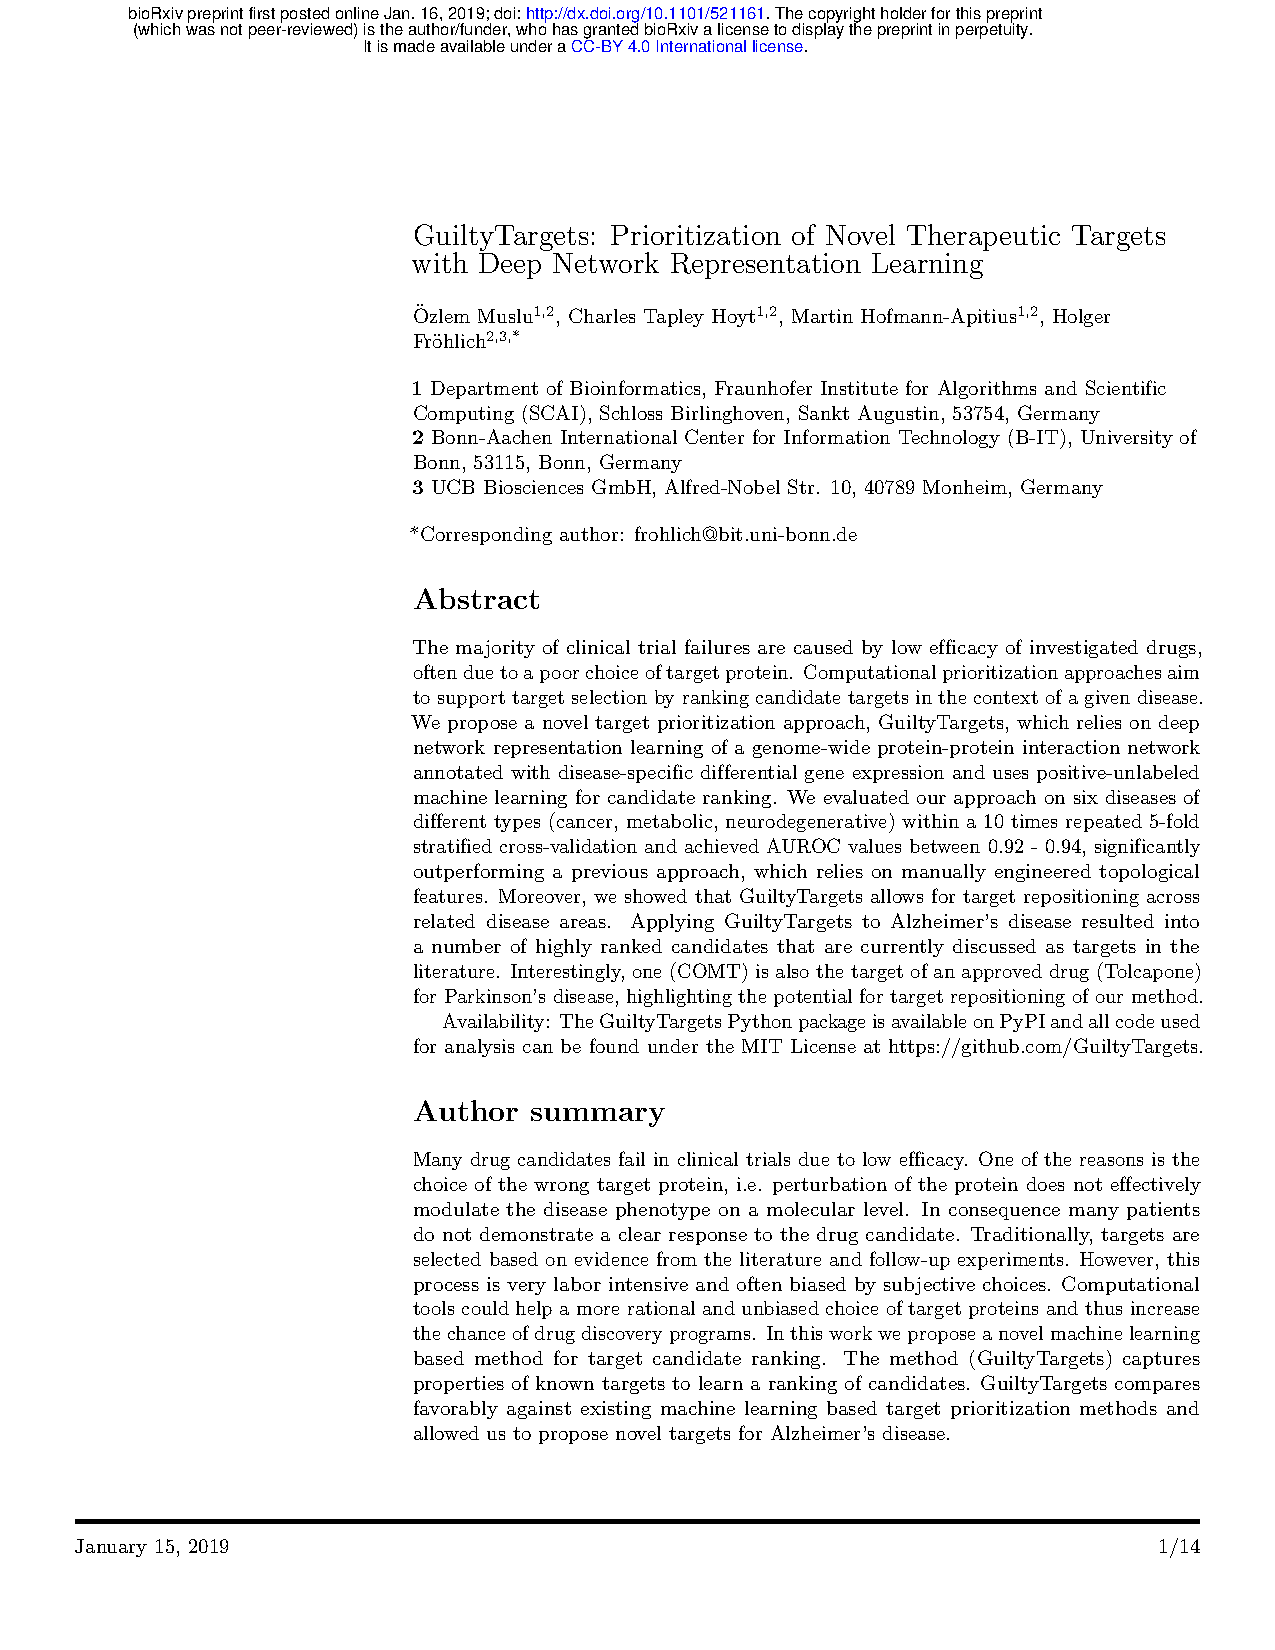
\includepdf[pages={-}]{articles/guiltytargets.pdf}

\section*{Postface}

The exchange of engineered topological features for learned features increased the performance in target prioritization across nearly all combinations of protein-protein interaction databases (i.e., HIPPIE and STRING), disease-target association databases (i.e., Therapeutic Target Database and OpenTargets), and other hyperparameters used in the workflow from Emig \textit{et al.}~\cite{Emig2013}.

The work of Emig \textit{et al.} was careful to validate using a variety of diseases that were well understood.
Following validation and comparison to Emig \textit{et al.}, this publication turns towards applications to neurodegenerative disease---an indication notorious for poor choice of target proteins during drug discovery.
The most infamous is the amyloid beta precursor protein due to the ubiquity of aggregates of its cleavage products, A$\beta$40 and A$\beta$42 in the brains of \ac{AD} patients.
However, all clinical trials until this point targeting this protein have failed.
GuiltyTargets proposed new targets that have not been previously clincally investigated in the context of \ac{AD} such as CHRNB4, a nicotinic receptor subunit for which there is mounting epidemiological evidence of the importance in the disease.

While GuiltyTargets comprises a machine learning pipeline for node-based prioritization of targets in knowledge graphs, future work will incorporate other sources for automatically contextualizing these targets with their related druggability, side effects, and clinical trial landscape.
The same workflow in which network representation learning is used to replace topological features could be used to improve upon previous drug repositioning efforts such as~\cite{Himmelstein2017}.
While initial work used the same protein-protein interaction networks and disease-specific differential gene expression profiles, it can be extended to accommodate the rich knowledge encoded in \ac{BEL} networks generated by manual, semi-automated, and automated approaches described elsewhere in this thesis.
Several respective master's theses found at \url{https://github.com/lingling93/comparison}, \url{https://github.com/aldisirana/SE_KGE}, and \url{http://github.com/guiltytargets/phewas} are in progress investigating these questions.
Future work could also easily incorporate the networks arising from Bio2BEL packages presented in Chapter~\ref{ch:bio2bel}.
